
\documentclass[sigconf, anonymous]{acmart}
%%
%% \BibTeX command to typeset BibTeX logo in the docs
\AtBeginDocument{%
  \providecommand\BibTeX{{%
    Bib\TeX}}}
\let\Bbbk\relax
\usepackage{threeparttable}
\usepackage{amsmath,amssymb,amsfonts}
\usepackage{algorithm}
\usepackage{algpseudocode}
\usepackage{graphicx}
\usepackage{textcomp}
\usepackage{subcaption}
\usepackage{booktabs}
\usepackage{url}
\usepackage{colortbl}
\usepackage{xcolor}

\setcopyright{acmlicensed}
\copyrightyear{2026}
\acmYear{2026}
\acmDOI{XXXXXXX.XXXXXXX}
%% These commands are for a PROCEEDINGS abstract or paper.
\acmConference[e-Energy'26]{17th ACM International Conference on Future and Sustainable Energy Systems}{June 22--25,
  2026}{Banff, CN}

%% Added macros
\newcommand{\minimize}{\text{minimize}}
\newcommand{\subjectto}{\text{subject to}}
\newcommand{\edit}[1]{{\color{red}#1}} 
\newcommand{\proj}{\mathbf{proj}}

\begin{document}
\title{On the Grid: Differentiable }

% \author{Grant Wilkins}
% \authornotemark[1]
% \email{gfw@stanford.edu}
% \affiliation{%
%   \institution{Stanford University}
%   \city{Stanford}
%   \state{CA}
%   \country{USA}
% }

% \author{Akshay Sreekumar}
% \authornote{Both authors contributed equally to this research.}
% \email{akshay81@stanford.edu}
% \affiliation{%
%   \institution{Stanford University}
%   \city{Stanford}
%   \state{CA}
%   \country{USA}
% }

% \author{Fiodar Kazahmiaka}
% \email{fkazhamiaka@microsoft.com}
% \affiliation{%
%   \institution{Microsoft, Inc.}
%   \city{Redmond}
%   \state{WA}
%   \country{USA}
% }

% \author{Ram Rajagopal}
% \email{ramr@stanford.edu}
% \affiliation{%
%   \institution{Stanford University}
%   \city{Stanford}
%   \state{CA}
%   \country{USA}
% }

\renewcommand{\shortauthors}{Anonymous et al.}

\begin{abstract}

The rapid expansion of AI computing infrastructure has led to datacenter interconnection requests at an unprecedented rate, with individual campuses now proposed at the many gigawatt scale. These large loads can cause congestion, raising locational marginal prices (LMPs) and systemwide operating costs; effects that can be socialized to other regional consumers.

We develop a framework for stress-testing large-load placement decisions that couples datacenter capacity allocation with network-constrained dispatch. We treat distributed siting as a load-side lever to manage congestion, in contrast to typical grid-side levers such as transmission and generation expansion. Using a bilevel optimization formulation that minimizes dispatch costs and LMPs, we evaluate how optimally distributing capacity across candidate buses affects datacenter capital expenditure, grid upgrades, and congestion. We apply the framework to a 101-bus representation of the U.S. Western Interconnection from PyPSA-USA under load injections ranging from hundreds of megawatts to multiple gigawatts, with varied workload-characteristic profiles.

Our results reveal sensitivities in placement, as adding capacity with certain load profiles at specific locations can trigger sharp LMP increases once critical transmission constraints bind. Distributing load across multiple sites reduces peak LMP impacts by over 42.6\% compared to single-site injection at equivalent capacity. Combining distributed placement with grid-side levers enables deploying 1 GW more datacenter capacity before the same constraints bind. Finally, differences in workload profiles -- e.g., training vs. inference -- can materially alter optimal placements, motivating scenario-based stress testing as a necessary planning tool.
\end{abstract}

\keywords{Grid, Computing}
\maketitle

\section{Introduction}

\begin{figure}
    \centering
    \begin{subfigure}[b]{\columnwidth}
        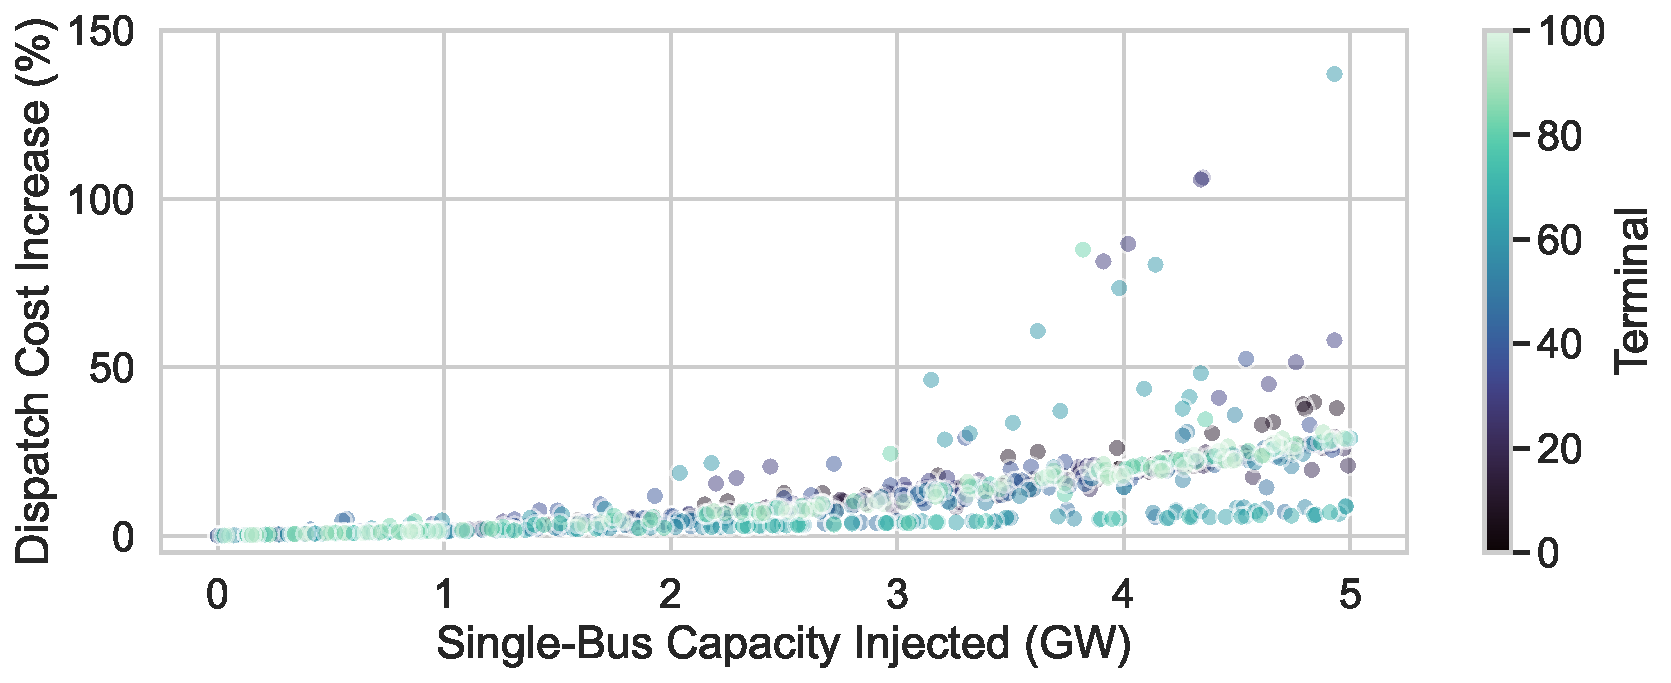
\includegraphics[width=\linewidth]{figures/dispatch_cost_percent_increase.pdf}
        \caption{Dispatch cost increase.}
        \label{fig:dispatch-cost-cloud}
    \end{subfigure}
    \begin{subfigure}[b]{\columnwidth}
        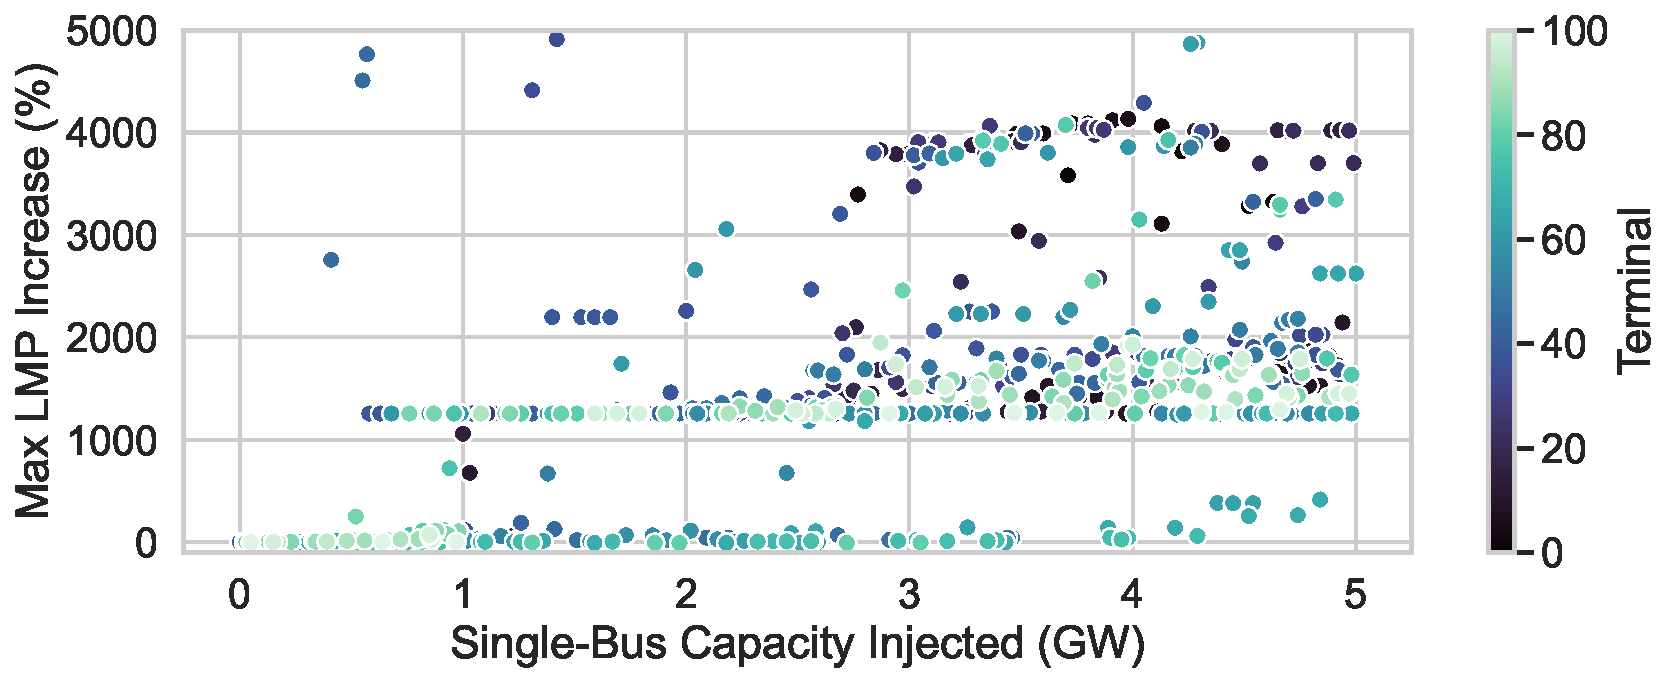
\includegraphics[width=\linewidth]{figures/max_lmp_increase.pdf}
        \caption{Max locational marginal price (LMP).}
        \label{fig:max-lmp-cloud}
    \end{subfigure}
    \caption{Dispatch and locational marginal price (LMP) for WECC when provisioning a data center load at a single terminal. We notice that in general, the cost of operating the system and LMP rises with increasing capacity.}
    \label{fig:cloud-plots}
\end{figure}

\textbf{Motivation.} The rapid expansion of AI computing infrastructure has led to requests for electric load connection at an unprecedented rate. 
Individual data-center campuses are now proposed at
hundreds of megawatts to gigawatt scale~\cite{stargate, gw-scale}, with interconnection requests arriving
on compressed timelines and often concentrated at a small number of transmission buses~\cite{EPRI2024PoweringDataCenters, dukerethinking}. As a result, the planning question facing system operators and regulators is no longer only whether sufficient generation exists to serve new demand, but \emph{where} large loads should be connected and how concentrated those connections should be across the network.

Public concerns around large datacenter interconnections often center around sustainability~\cite{},
rate hikes~\cite{}, and downstream cost impacts for other consumers~\cite{}. These effects arise through known
mechanisms. Changes in congestion and dispatch induced by large-load siting decisions 
are seen in the system as higher locational marginal prices (LMPs) and total 
dispatch costs. When a new load activates transmission constraints, system operators 
must redispatch generation away from least-cost units toward more expensive marginal 
resources. This raises systemwide dispatch costs and increases LMPs at constrained 
locations, with effects that can extend well beyond the bus where the load was added. 
LMPs are not prices paid by the consumer, but instead signs that point towards 
potentially higher rates. Large load owners, such as data-center operators, are 
exposed directly through nodal energy prices and congestion charges. Other consumers may be affected indirectly via congestion cost allocation or rate increases that recover higher system operating costs over time. 


While these effects are well
studied in economic planning, existing work has not been used to compare 
alternative load placement strategies for the same aggregate demand. As data-center 
demand scales from tens of megawatts to multiple gigawatts, this limitation becomes 
more pronounced.

A central challenge our work demonstrates is that a grid's response to new load is highly nonlinear. Adding capacity at some
locations can be absorbed with modest impact on the system at large, while similar additions elsewhere can
trigger congestion and price escalation once specific transmission constraints or critical lines bind. These ``knee''
points are location-dependent and are not visible in traditional peak/off-peak screening studies. 
As one can see in Figure~\ref{fig:cloud-plots} both LMPs and dispatch cost increase 
system-wide no matter where a datacenter is placed. For LMPs in Figure~\ref{fig:max-lmp-cloud}, 
some nodes do exist in the bottom right regime with a low change in price with added 
capacity, yet the vast majority of nodes see a massive increase in LMP.


In this study, we develop a framework for stress-testing large datacenter load siting
decisions. Rather than proposing a single optimal placement, we evaluate how alternative allocations of
a fixed interconnection capacity across candidate buses affect system dispatch cost, LMP distributions,
and congestion patterns under operation. We explicitly distinguish provisioned utility-side interconnect capacity from normalized temporal load profiles, enabling apples-to-apples
comparison across different capacity concentrations and site counts. The framework emphasizes
diagnostics, such as changes in the set of binding transmission constraints, to explain why
distribution helps in some regimes and fails in others.

We apply the framework to a 101-bus representation of the U.S. Western Interconnection and study
large-load injections ranging from tens of megawatts to multiple gigawatts. Our results reveal....

Our contributions are as follows.
\begin{enumerate}
    \item We produce a comparative framework for evaluating large-load siting strategies that quantifies congestion, dispatch-cost, and LMP impacts.
    \item We demonstrate that distributing large loads across multiple nodes can mitigate LMP spikes as compared to single site injection.
    \item We explore how distribution of load with other grid levers such as transmission upgrades and extra storage can improve the amount of deployable capacity.
    \item We compare our proposed optimization framework to that of naive baselines demonstrating that we are able to offset the pricing and congestion effects through distributed placement.
    \item We quantify the ways in which workload differences and different site load profiles can lead to regret and optimality gap's in placed data centers.
\end{enumerate}


% \section{Background}
\section{Background and Motivation}

\subsection{Data Center Growth and Electricity Pricing}
\edit{BY AKSHAY, GRANT TAKE A LOOK}
The recent growth of large scale data center loads has become a focal point in public discourse surrounding electricity pricing and grid upgrades. The determination of retail rates is multi-factorial, influenced by tariffs, fuel prices, regulatory decisions, infrastructure investments, and resource adequacy procurements. Still, the impacts of large load siting decisions in the wholesale market have long reaching effects that may impact consumers. 

The injection of large loads at specific locations on the grid can trigger congestion driven redispatch. By altering power flows, new load can cause transmission constraints to bind, requiring the operator to redispatch generation away from cheaper units to more expensive marginal resources. This can increase system operating costs and raise \emph{locational marginal prices (LMPs)} at nodes affected by the induced congestion. Although LMPs are wholesale settlement prices rather than retail tariffs, they are an indicator of congestion making load more expensive to serve. Other large loads may be exposed directly to these higher nodal energy prices, while consumers can be affected indirectly through rate adjustments that seek to recover higher system costs over time. Large load interconnection is often accompanied by additional infrastructure costs (e.g. transmission expansion) to handle congestion, and these costs may also be socialized among ratepayers. 

Of course, attributing changes in retail rates directly to a specific load interconnection is not possible. However, it is important to understand how siting large data center loads contributes to changing congestion patterns and system-wide pricing signals that may be directionally consistent with increased downstream cost pressure. Addressing this question requires a careful evaluation of the system as a whole, as congestion and redispatch effects can propagate non-locally across the network. 

\subsection{Existing Data Center Planning Practices}
Large load planning on transmission networks typically evaluates system reliability through stressed-case snapshots (e.g., peak and off-peak conditions) to ensure voltage bounds, thermal limits, and stability margins are maintained~\cite{nerc_tpl001_5.1}. This approach treats loads as a capacity requirement and asks whether sufficient headroom exists to serve it reliably, assuming other siting and regulatory features have already been met. Datacenter siting decisions, in turn, prioritize power availability, land cost, fiber connectivity, and natural disaster risk, treating the grid as a constraint to satisfy rather than a system whose behavior changes with placement~\cite{goiri2011intelligentplacement,ALAPERA201869}. While grid-side planners consider some congestion effects, neither process systematically can quickly evaluate how different mechanics of load injection affect congestion patterns, wholesale market pricing, or dispatch costs; these variables depend jointly on where capacity connects, how much is injected, and when demand occurs. Recent NERC guidance acknowledges this gap, noting that the operational behavior of emerging large loads like datacenters can induce new risks that fall outside of the previous ranges; recommending that planners should explore several new strategies and load patterns~\cite{nerc2026}. It has been well documented that AI workloads prevalent in these new large loads exhibit fast, large variability across training and inference phases~\cite{chen2025electricitydemandgridimpacts, patel2024llms, li2024unseenaidisruptionspower, dynamollm}. This variance implies that the same provisioned MW can produce materially different grid congestion and pricing effects depending on workload mix. Our framework addresses these limitations by coupling temporal load profiles with planning and dispatch levers to allow for an evaluation of placement strategies under these different operational conditions.

\subsection{Mitigation Levers}

There are a plethora of conventional planning interventions to mitigate the impacts of connecting large data center loads—building or upgrading transmission infrastructure, expanding generation resources, or curtailing loads. These levers are invaluable tools in managing the health of the grid, but can also be slow and capital intensive. Additionally, many of these levers are positioned as \emph{system} upgrades in \emph{response} to an interconnection request, rather than as a design variable on the load side. 

We posit that the \emph{distribution} of large data center loads offers a load-side lever that can be used in conjunction with more traditional planning levers. By choosing where to concentrate loads on the grid, siting decisions act as a way to reduce externalities such as peak-price events without requiring immediate system-wide upgrades or reducing the magnitude of such upgrades. Distribution can reduce the burden of congestion costs and redispatch impacts, which may translate into lower wholesale exposure for the data center operator and lower long-term cost pressure for the system as a whole. 

This additional planning tool comes with important caveats. Distributed placement can increase a data center operator's operational complexity, with additional care required to handle latency constraints, supply-chain logistics, and land acquisition. Load curtailment and flexible operation are also possible options to mitigate the effects of data center loads, but deploying these options reliably at a large-scale requires additional study which is out of the scope of this work. 

We emphasize that distribution as a load-side lever is meant to be used alongside other planning levers. Distributed interconnection paired with transmission expansion or storage deployment may reduce the magnitude of upgrades required to service the same aggregate demand. Considering load placement as complementary to other grid invests can ``shift the knee" in price response curves, thereby expanding the range of demand levels that can be served without severe price spiking. 

% \subsection{Capacity Expansion Modeling}
% Capacity expansion problems, and more specifically bilevel capacity expansion problems, have a rich literature, particularly from the perspective of planning grid infrastructure investments. A well-studied class of problems closely related to our setting is \textit{profit maximization}, where merchant investors plan new generation investments with the goal of maximizing market profits while accounting for the need to upgrade transmission infrastructure when necessary. In these models, investors seek to favorably influence market outcomes while minimizing expenditures on costly grid reinforcements \cite{baringo2011wind, wogrin2011generation}.

% These problems are naturally thought of as bilevel optimization problems and can be viewed as a type of Stackelberg game, where a leader (the investor) anticipates the market clearing outcome (the follower). In general, bilevel expansion problems are highly nonconvex and computationally challenging. Classical approaches aim to find globally optimal solutions by first reformulating the problem as a Mathematical Program with Equilibrium Constraints (MPEC). These MPECs can then be further reformulated as mixed-integer programs (MIPs) that are solvable with commercial solvers such as Gurobi \cite{gurobi2025}. While this approach theoretically enables exact solutions, it comes at a significant computational cost. Bilevel expansion problems are known to be NP-hard, and solving large MIP formulations to global optimality quickly becomes infeasible, particularly when the planner wishes to evaluate a large number of scenarios with varying system conditions and uncertainty realizations.

% In this work, we use the gradient-based methods for bilevel expansion planning introduced in \cite{degleris2024gradient}, which aim to find high-quality, locally optimal solutions much more efficiently than traditional MIP-based approaches. Gradient methods avoid the combinatorial explosion associated with MPEC reformulation and instead directly leverage the structure of the bilevel problem to enable scalable optimization. Given the complex, coupled constraints associated with data center buildout—including grid infrastructure limitations, quality-of-service (QoS) requirements, and capital expenditure (CapEx) considerations—it is critical that the planner can quickly iterate over many candidate scenarios to identify acceptable and actionable planning solutions.


% \subsection{Data Center Power and Siting Constraints}
% Prior work has extensively studied power modeling and planning for data centers, though typically without considering the broader grid context that our approach addresses. Power distribution hierarchies in data centers involve multiple distribution paths for high availability and fault tolerance~\cite{hsu2018smoothoperator,zhang2021flex, wu2016dynamo}. Investment decisions in placement of resources are therefore made at a rack level due to the capital expenditures required for the surrounding infrastructure. Beyond the actual hardware, workload characterization like in Coach~\cite{reidys2025coach}, DynamoLLM~\cite{dynamollm}, and POLCA~\cite{patel2024llms}, demonstrated that general data center and AI inference workloads exhibit temporal patterns with complementary usage across different applications, making them suitable for strategic placement and oversubscription. Although these works provide valuable information on internal data center power management and workload characterization, they do not address the cross-layer optimization between data center placement and grid capacity expansion that our approach aims to achieve.

% \subsection{Cost Concerns for Large Datacenter Loads}
% A recent discussion in news and government has concerned the harmful
% effects of data centers on local communities, namely the rising cost
% in electric utility bills. While there are many confounding variables,
% adding large data center loads to areas does have the potential to
% drive up costs for residential and other commercial consumers, as
% often grid upgrades are socialized 


\section{Problem Setting}

\subsection{Bilevel Capacity Expansion Planning}
Following \cite{degleris2024gradient}, we specify the general bilevel expansion planning problem as
\begin{equation}
\begin{aligned}
\minimize\quad & \gamma^\top \eta + h(z^{\star}\left(\eta)\right) \\
\subjectto\quad & \eta \in \mathcal{E},
\end{aligned}
\label{eq:bilevel_problem}
\end{equation}
where $\eta \in \mathbb{R}^K$ are the design variables representing capacities of power system components and $\gamma \in \mathbb{R}^K$ defines the linear investment costs associated with expanding those capacities. The function $h: \mathbb{R}^N \to \mathbb{R}$ represents the planner's operational objective. The set $\mathcal{E}$ denotes the constraints on the expansion plan, which in our case are typically box or budget constraints on $\eta$.

The term $z^{\star}(\eta)$ denotes the \emph{solution map} of the dispatch problem, giving the optimal primal and dual variables expressed as a function of the expansion plan. Formally, we define $z^{\star}(\eta) = (p^{\star}, v^{\star}, \lambda^{\star}, \omega^{\star}, \mu^{\star})$, comprising power injections $p$, phase angles $v$, and dual variables $\lambda$, $\omega$, and $\mu$ associated with the dispatch constraints. We now describe the dispatch problem.

\subsection{Dispatch Model}
The lower level optimization problem in the bilevel framework is the dispatch problem, formulated as DC Optimal Power Flow (DC-OPF). We require that the solution map $z^{\star}(\eta)$ be differentiable with respect to the data center capacities. The dispatch problem is given by:
\begin{equation} \label{eq:dc-opf-full}
\begin{array}{llr}
    \text{minimize} \quad 
    & \sum_d c_d(p_d, v_d; \theta_{d}) \quad\\
    \text{subject to} \quad 
    & \sum_d A_d p_d = 0,
        \quad\quad & (\lambda) \\
    & A_d^T v_d = u, \quad d = 1, \ldots, D & (\omega_d)
\end{array}
\end{equation}
where $c_{d}$ represents the cost function of device $d$ in the network, $p_{d}$ are the associated power injections, and $v_{d}$ are the phase angles. The parameters $\theta_d$ capture device-specific data such as capacity limits and marginal costs. The dual variables $\lambda$ and $\omega_{d}$ correspond to the power balance and device coupling constraints, respectively.

Additional operational constraints, such as transmission line flow limits, are encoded implicitly within the device cost functions $c_d$. For example, a transmission line's cost function includes indicator terms that enforce flow limits, with associated dual variables $\mu_\ell^+$ and $\mu_\ell^-$. Similarly, generator capacity bounds enter through the generator cost functions. This device-oriented formulation, implemented in Zap \cite{degleris2024gpu}, maintains differentiability of the solution map while capturing standard network constraints. For further details, the reader is referred to \cite{degleris2024gpu}.

\subsection{Base Problem Formulation}
In this work, we consider several different instances and variants of Problem \ref{eq:bilevel_problem} to understand how different siting decisions and mitigation levers interact. 

In the base data center planning experiment, we allocate a fixed data center interconnect capacity across a set of candidate buses. We assume that these candidate buses are a fixed subset of all the buses in the network, and that they have been selected based on multiple criteria such as land cost, regulatory concerns, and logistics. Given this, we ignore the linear investment cost term in our base planning experiment, choosing to calculate it after the fact. This reflects limitations in planning flexibility where we know data centers must sit at one of a few proposed sites (already screened for cost), and we are interested in choosing from among the best of these possible options. We solve

\begin{equation}
\begin{aligned}
\minimize\quad &  h_{\text{LMP}}(z^{\star}\left(\eta)\right) \\
\subjectto\quad & \eta \in \mathcal{E}_{\text{DC}},
\label{eq:dc_plan}
\end{aligned}
\end{equation}

where $\eta \in \mathbb{R}^K$ now represents the data center capacity allocated across each of $K$ candidate locations, and $h_{\text{LMP}}$ is an objective related to the LMPs in the system. More formally, we have

\begin{equation}
\begin{aligned}
h_{\text{LMP}}(\Lambda)
&=
\beta \sum_{t=1}^{T}\frac{1}{\alpha}\log\!\left(\sum_{i=1}^{N}\exp\!\left(\alpha\,\Lambda_{i,t}\right)\right),
\end{aligned}
\label{eq:h_lmp}
\end{equation}

where $\Lambda \in \mathbb{R}^{N \times T}$ is the matrix of nodal LMPs across the $N$ buses in the system for a time horizon of $T$ steps. The function $h_{\text{LMP}}$ is a sum of the smooth maximums of the system LMPs, with $\alpha \in \mathbb{R}$ controlling the smoothness of the approximation, and $\beta$ acting as a scaling factor to control the magnitude of the objective. 

In the base experiment, we define the constraint set as

\begin{equation}
\begin{aligned}
\mathcal{E}_{\text{DC}}
\;:=\;
\Bigl\{
\eta \in \mathbb{R}^{K}
\;\Big|\;
\underline{\eta} \le \eta \le \overline{\eta},\;
\mathbf{1}^\top \eta = B
\Bigr\}.
\end{aligned}
\end{equation}

where $\underline{\eta}$ and $\overline{\eta}$ represent lower and upper bounds on data center capacity at a site, while $B$ is the total amount of allocated data center capacity. We note that solving Problem \ref{eq:dc_plan} gives us an expansion plan for data center capacities optimized to control the effects of pricing peaks in the system. Problem \ref{eq:dc_plan} also permits a wide design space, with variables such as the number of sites $K$, the total budget $B$, and the box constraints $(\underline{\eta}, \overline{\eta})$ allowing us to model different scenarios and optimal allocations. 

We also utilize the form of Problem \ref{eq:bilevel_problem} to plan transmission and generation expansion as mitigation levers. For these, we solve

\begin{equation}
\begin{aligned}
\minimize\quad & \gamma^{\top}\eta + h_{\text{dispatch}}(z^{\star}\left(\eta)\right) \\
\subjectto\quad & \eta \in \mathcal{E},
\label{eq:grid_expansion}
\end{aligned}
\end{equation}

where $h_{\text{dispatch}}(z^{\star}(\eta))$ returns the dispatch cost (i.e., the objective of Problem \ref{eq:dc-opf-full}) and $\gamma^{\top}\eta$ reflects the investment cost of expanding transmission or generation. The constraint sets for transmission and generation are

\begin{equation}
\begin{aligned}
\mathcal{E}_{\text{trans}}
\;:=\;
\Bigl\{
\eta \in \mathbb{R}^{L}
\;\Big|\;
\eta^{0}_{\text{L}} \le \eta \le \overline{\eta}_{\text{L}}
\Bigr\},
\end{aligned}
\end{equation}

\begin{equation}
\begin{aligned}
\mathcal{E}_{\text{gen}}
\;:=\;
\Bigl\{
\eta \in \mathbb{R}^{G}
\;\Big|\;
\eta^{0}_{\text{G}} \le \eta \le \overline{\eta}_{\text{G}}
\Bigr\},
\end{aligned}
\end{equation}

where $L$ is the number of transmission lines and $G$ is the number of generators. The lower bounds $\eta^{0}_{\text{L}}$ and $\eta^{0}_{\text{G}}$ represent existing capacity, reflecting that we are expanding (not retiring) infrastructure. The upper bounds are parameterized by expansion factors $\epsilon_{\text{L}}$ and $\epsilon_{\text{G}}$ relative to existing capacity, i.e., $\overline{\eta}_{\text{L}} = (1 + \epsilon_{\text{L}}) \cdot \eta^{0}_{\text{L}}$ and $\overline{\eta}_{\text{G}} = (1 + \epsilon_{\text{G}}) \cdot \eta^{0}_{\text{G}}$.

We note that the expansion planning objectives are \emph{different} for data center expansion versus conventional transmission and generation expansion. Transmission and generation expansions are system upgrades, possibly triggered by large load interconnection, where the operator's objective is to benefit the system by minimizing investment and dispatch cost. Data center capacity is not a system upgrade, and so our objective instead mitigates negative externalities (i.e., price spikes) associated with the interconnection.


% \section{Problem Formulation}
\label{sec:problem}

Let the transmission network contain a finite set of buses
$\mathcal{N}$ and let $\mathcal{K}\subseteq\mathcal{N}$ denote the
\emph{candidate} buses identified via the node-selection heuristic
in Section~\ref{sec:node-selection}. The planner allocates a
total capacity budget $C\;[\mathrm{MW}]$ across $K=|\mathcal{K}|$ sites.
The continuous decision variables $\boldsymbol{\eta}\in\mathbb{R}_{+}^{K}$
specify the nameplate IT capacity $\eta_k$ assigned to each site $k$.

Data center power consumption depends on the application mix~\cite{patel2024llms}.
We consider a set of \emph{workload scenarios} $\mathcal{S}$
representing distinct operational profiles -- for example,
inference-dominated deployments with diurnal demand patterns~\cite{dynamollm}
versus training-dominated deployments with sustained high
utilization and periodic synchronization transients~\cite{stabilization}.
Each scenario $s \in \mathcal{S}$ is characterized by a
normalized load-factor trace $\boldsymbol{\ell}_s \in [0,1]^T$
over $T$ time periods; the power injected at site $k$
under scenario $s$ is then
$P_{k,s}(t) = \eta_k \cdot \ell_s(t)$.
Section~\ref{sec:workload} details how these traces are generated.

\noindent\textbf{Bilevel optimization model.} Following \citet{degleris2024gradient}, the \textit{upper level} of our planner minimizes
investment cost plus expected operating cost:
\begin{equation}
\label{eq:upper}
\min_{\boldsymbol{\eta}\ge 0}\;
  \boldsymbol{\gamma}^{\!\top}\boldsymbol{\eta}
  + \sum_{s\in\mathcal{S}} w_s\, h_s\bigl(x_s^\star(\boldsymbol{\eta})\bigr)
\quad\text{s.t.}\;\;
  \mathbf{1}^{\!\top}\boldsymbol{\eta}=C,
\end{equation}
where $\boldsymbol{\gamma}\in\mathbb{R}_{+}^{K}$ is the site-specific
capital cost (Section~\ref{sec:investment-cost}), $w_s$ are
scenario weights summing to one, and $h_s(\cdot)$ extracts
total generation cost from the dispatch solution.

Then, the \textit{lower level} of our model performs economic dispatch.
Given our fixed $\boldsymbol{\eta}$, each scenario $s$ solves a
network-constrained optimal power flow:
\begin{equation}
\label{eq:lower}
x_s^\star(\boldsymbol{\eta})
= \arg\min_{p,\theta}\;
  \sum_{g \in \mathcal{G}} c_g(p_g)
\end{equation}
where $p_g$ is generation from unit $g$, $c_g$ is its cost curve,
and $\theta$ are voltage angles determining line flows.
Data center loads enter as fixed withdrawals at their assigned buses.
The dispatch model, implemented via Zap~\citep{degleris2024gpu},
is differentiable in $\boldsymbol{\eta}$, enabling gradient-based
solution of~\eqref{eq:upper}.

% \section{Methods: Our Modular Approach}\label{sec:methods}
\section{Methods}

\subsection{Planning Pipeline Overview}
\edit{GRANT TO MAKE FIGURE}

Figure \ref{fig:pipeline_overview} shows the high level overview of determining an optimal data center capacity allocation within our framework. We leverage Zap, an open-source Python package for differentiable electricity systems modeling, to formulate and solve both the bilevel capacity expansion planning problem in (\ref{eq:dc_plan}) and the underlying dispatch model given in (\ref{eq:dc-opf-full}). A full Zap planning instance is specified given power network data, data center workload models, a set of candidate interconnection sites, and problem data ($\mathcal{E}$, $h$, $\gamma$).

To generate the underlying power network data needed for a Zap instance, we use PyPSA-USA \cite{tehranchi5029120pypsa} to generate a realistic model of the U.S. Western Interconnection (WECC). PyPSA-USA provides an open-source modeling platform built on top of PyPSA that enables high spatial and temporal resolution modeling of generation, storage, and transmission infrastructure across the continental United States. We give a detailed description of our PyPSA network model in Section \ref{sec:pypsa_network}. We provide details for the candidate set construction and the workload models below. 

\subsection{Cost Models}\label{sec:investment-cost}
One of the primary variables to compare different levers against is cost. However, cost can be a complicated variable to reason about due to the different owners of assets and time scales over which acquisition takes place. For simplicity, we treat all costs as annualized over 20 years with a 7\% discount rate, meaning that all costs are represented as annual investment and not total nameplate costs. Investment 

\noindent\textbf{Datacenter build-out cost.} For each candidate bus $k \in \mathcal{K}$ we 
assign a power-normalized site cost $\gamma_k$ (\$/MW) that enters the upper-level objective in
Equation~\eqref{eq:upper}. Reported hyperscale datacenter development costs
(often expressed per MW of critical IT load) commonly fall in the range
\$9--15M/MW~\cite{CushWakeCostGuide_2025}, with variation due to 
environmental variables, electrical design, cooling requirements, and other
choices~\cite{stojkovic2025rearchitectingdatacenterlifecycleai}.
To mitigate this variance, we model site cost as a fixed construction 
baseline plus a location-specific land term:
\begin{equation}\label{eqn:investment-cost}
    \gamma_k = \Gamma_{\text{build}} + A_{\text{MW}} \cdot P^{\text{land}}_k.
\end{equation}
We set $\Gamma_{\text{build}} = \$12$M/MW (median of the above range), and
compute $P^{\text{land}}_k$ by mapping each bus's FIPS county code to an
estimated land value surface~\cite{land-cost}. To relate land area to 
provisioned capacity, we use recommended hyperscaler site and power sizes to 
set $A_{\text{MW}} = 0.25$ acres per MW. We then show 
robustness as a sensitivity parameter \cite{stream_landowners_2025}.

\noindent\textbf{Transmission expansion cost.}\edit{ADD TRANSMISSION COSTS} When enabling transmission expansion, we allow a subset of
lines to be added with their corresponding investment costs to the
planning objective. We use the PyPSA-USA default annualized transmission expansion costs which are parameterized as a function of length and MW capacity
and are derived from NREL ReEDS transmission cost assumptions~\cite{nrel-reeds, tehranchi5029120pypsa}. 
Following prior work using the same dataset, we take expansion costs directly 
from the dataset and scale capital costs to the simulated horizon~\cite{degleris2024gradient}.

\noindent\textbf{Generator upgrade cost.} \edit{ADD GENERATOR ASSUMPTIONS}

\noindent\textbf{Dispatch cost.} \edit{ADD DISPATCH COSTS} As previously discussed, Zap solves the dispatch problem based on the planned PyPSA devices. Dispatch cost is the cost of operating the grid by supplying generation to all loads over the course of the simulated day 



\subsection{Candidate Set Construction}
\edit{GRANT WRITE THIS}

* Start with a realistic candidate list (not “any bus”)
  * proxy constraints: land, zoning, proximity to infrastructure, etc.
* Heuristics we already use:
  * generation-rich / existing-load ranking
  * cheapest land nodes, etc.
* Why it matters:
  * avoids curious placements that win out because of missing constraints
* Firmly state that many such candidates exist and we limit to some for DC operator operational simplicity
  * further, we are pinning land cost and value to the FIPS code from PyPSA for the transmission bus
  * not indicative of an actual site, but instead just where the interconnect would be
  * land price from (2020) work and is a fuzzy estimator for site value
  * assuming some other ~0.56MW/Acre (Cushman Wakefield), 1.3x inflation adjuster (Fed), and \$12.5M/MW (Cushman Wakefield)

\subsection{Workload Scenario Modeling}\label{sec:workload}
\edit{GRANT REFINE THIS}
Our framework evaluates how adding a large load at bus $k$ alters both operating outcomes
(dispatch cost, congestion, and LMPs) and siting decisions. To do so, we represent each
workload scenario $s \in \mathcal{S}$ as a normalized demand profile $\ell_s(t)\in[0,1]$ over the study
horizon $t=1,\dots,T$ (every 15 mins). The decision variable $x_k$ denotes the
provisioned \emph{utility/interconnect} capacity (MW) at bus $k$, and the realized demand injected
into the dispatch model is
\begin{equation*}
p_{k,s}(t) = x_k \, \ell_s(t).
\end{equation*}
This construction allows a single set of shape traces $\{\ell_s(t)\}$ to be scaled to alternative
provisioned capacities and compared on equal footing.


Existing transmission planning practice often emphasizes a small set of snapshot conditions
(e.g., peak and off-peak cases). Recent reliability guidance cautions that the operational behavior of
emerging large loads can induce risks outside of traditional peak/off-peak scenarios and recommends
that planners modify study assumptions and analyze a diversity of loading patterns~\cite{nerc2025largeloads, nerc2026}.
Therefore, we evaluate multiple workload shapes rather than a single peak-only
assumption.

We do not assume a single canonical ``AI'' load shape. Instead, to bound 
uncertainty and test how temporal characteristics interact with network 
constraints, we construct a small scenario set of (i) diurnal interactive 
profiles (representative of user-facing services, including inference-heavy 
front-ends), (ii) high-utilization sustained profiles (representative of long-
running, tightly coupled compute jobs), and (iii) ramp/step stress cases that 
capture rapid startup events or abrupt load loss as observed in HPC 
clusters~\cite{bates2015, shin2021revealing, patki2025global}. 
The goal is not to predict any operator’s exact utilization, but to demonstrate 
that plausible differences in temporal load shape can change which buses are 
attractive under the upper-level siting objective, as well as the downstream 
dispatch and LMP impacts under the same provisioned capacity.

\subsection{Solution Methods}

Solving Problem (\ref{eq:bilevel_problem}) requires choosing design variables $\eta$ (e.g. the allocation of interconnection capacity across candidate buses) subject to the convex constraints $\eta \in \mathcal{E}$. For any fixed choice of $\eta$, the system operations are given by solving the convex dispatch problem specified in Problem (\ref{eq:dc-opf-full}). The solution map of this problem is denoted by $z^{\star}(\eta)$. We denote the planning objective as 

\begin{equation}
    J(\eta) \;=\; \gamma^\top \eta \;+\; h\!\left(z^\star(\eta)\right),
    \label{eq:planning_objective_compact}
\end{equation}
where $\gamma^\top \eta$ captures linear investment costs and $h(\cdot)$ measures operational impacts of interest.

Although $h(z^\star(\eta))$ is defined implicitly through an optimization problem, the map $\eta \mapsto z^\star(\eta)$ is differentiable under standard regularity assumptions for convex programs. 

Consequently, $J(\eta)$ is differentiable, and minimizing~\eqref{eq:planning_objective_compact} reduces to a smooth optimization problem over a convex set. We therefore use \emph{projected gradient descent}, which iterates
\begin{equation}
\eta^{(i+1)} \;=\; \proj_{\mathcal{E}}\!\left(\eta^{(i)} - s \nabla J(\eta^{(i)})\right),
\label{eq:pgd_compact}
\end{equation}
with step size $s>0$.

Each gradient evaluation $\nabla J(\eta^{(i)})$ is computed by \emph{implicit differentiation} through the dispatch optimum. We solve the dispatch problem at $\eta^{(i)}$, then differentiate its KKT optimality conditions to obtain the sensitivity of $z^\star(\eta)$ to $\eta$. Zap provides an interface to to specify and solve planning problems via projected gradient descent. We refer the reader to \cite{degleris2024gradient} for the full derivation, convergence guarantees, and implementation details. 

% We give a brief overview of the gradient based methods used in Zap to solve the bilevel problems in (\ref{eq:bilevel_problem}) and (\ref{eq:dc_plan}). 

% Zap solves the bilevel Problems in (\ref{eq:dc_plan}) and (\ref{eq:dc_plan}) using gradient based methods. 

% Because we are able to differentiate through the solution map of the dispatch problem given in (\ref{eq:dc-opf-full}), we can compute the gradient of objective in (\ref{eq:dc_plan}) with respect to the capacities $\eta$. Thus, we leverage projected gradient descent to converge to a local solution of (\ref{eq:dc_plan}). More formally, we have 




% \subsubsection{Planning Objectives}

% We consider planning objectives of the following form. Formally, we follow \cite{degleris2024gradient} in specifying the bilevel optimization planning problem:

% \begin{equation}
% \begin{aligned}
%           \min_{\eta\ge0}\;\gamma^\top \eta + \sum_s w_s\,h_s\bigl(x_s^*(\eta)\bigr)
%           \quad\text{s.t.}\;\sum_i \eta_i = C
% \end{aligned}
% \label{eq:bilevel_problem}
% \end{equation}

% where \( \eta \in \mathbb{R}^K \) are the design variables representing data center capacities, \( \gamma \in \mathbb{R}^K \) defines the linear investment costs associated with the network capacities (this term captures the capital expenditure of expansion), and \( w_s \in \mathbb{R}_{++} \) are the scenario weights, which sum to one across all scenarios. The functions \( h_s : \mathbb{R}^N \to \mathbb{R} \) are the planner's operational objectives. While there are a multitude of different plausible planning objectives from the operational side, we consider minimizing the overall dispatch cost of the system. \(x_s^*(\eta)\) is the dispatch solution under data center addition \(\eta\). We additionally enforce the constraint that the total allocation of data center capacity must respect a capacity budget $C$.

% \subsection{Dispatch Model}

% The lower level optimization problem in the bilevel optimization framework is the following dispatch problem. We require that the solution map to the dispatch be differentiable with respect to the data center capacities. The dispatch problem is given by:

%     \begin{equation} \label{eq:dc-opf-full}
% \begin{array}{llr}
%     \text{minimize} \quad 
%     & \sum_d c_d(p_d, v_d; z_{d}) \quad\\
%     \text{subject to} \quad 
%     & \sum_d A_d p_d = 0,
%         \quad\quad & (\lambda) \\
%     & A_d^T v_d = u, \quad d = 1, \ldots, D& (\omega_d)
% \end{array}
% \end{equation}
% where $c_{d}$ represents the cost function of a device $d$ in the network, $p_{d}$ are the associated power flows, and $v_{d}$ are the phase angles. $\lambda$ and $\omega_{d}$ are the associated dual variables. Because we are able to differentiate through this problem, we can solve the Eq. \ref{eq:bilevel_problem} by running projected gradient descent, where we project onto the simplex to respect the allocation budget constraint. For more details, the reader is referred to \cite{ degleris2024gpu}.






\section{Experimental Setup}

\subsection{PyPSA Network and Calibration}
\label{sec:pypsa_network}

We use a model of the U.S. Western Interconnection from the historical year 2023 constructed using PyPSA-USA~\cite{tehranchi5029120pypsa} to run all of our experiments. Detailed generator, demand, and transmission representation is clustered to 101 terminals, 488 generators, 251 AC Lines, 3 HVDC links, 101 loads, and 52 batteries. The temporal resolution of the dataset is one hour. For our experiments, we consider the 24 hour time window for the day of 8/16/23 upsampled to a resolution of 15 minutes to better capture the granularity of the workload profiles. The dataset includes generator fuel costs, infrastructure capital costs, and maximum allowable renewable expansion limits. It also provides a realistic network model with line susceptances and capacity limits. Battery locations are included along with their corresponding energy and power parameters. 

We scale up all loads by $27\%$ and all generator capacities by $24\%$ to empirically match more recent capacity numbers in WECC \cite{eia or wecc or something}. We additionally scale down all transmission capacities by $30\%$ to simulate retirements and account for constrained network conditions under typical maintenance and new load addition.  

 


\section{Levers for Offsetting Cost}

\subsection{Distribution as a Load-Side Lever}
\label{sec:load_side_lever}

\begin{figure}[t]
  \centering


    \begin{subfigure}[t]{\columnwidth}
    \centering
    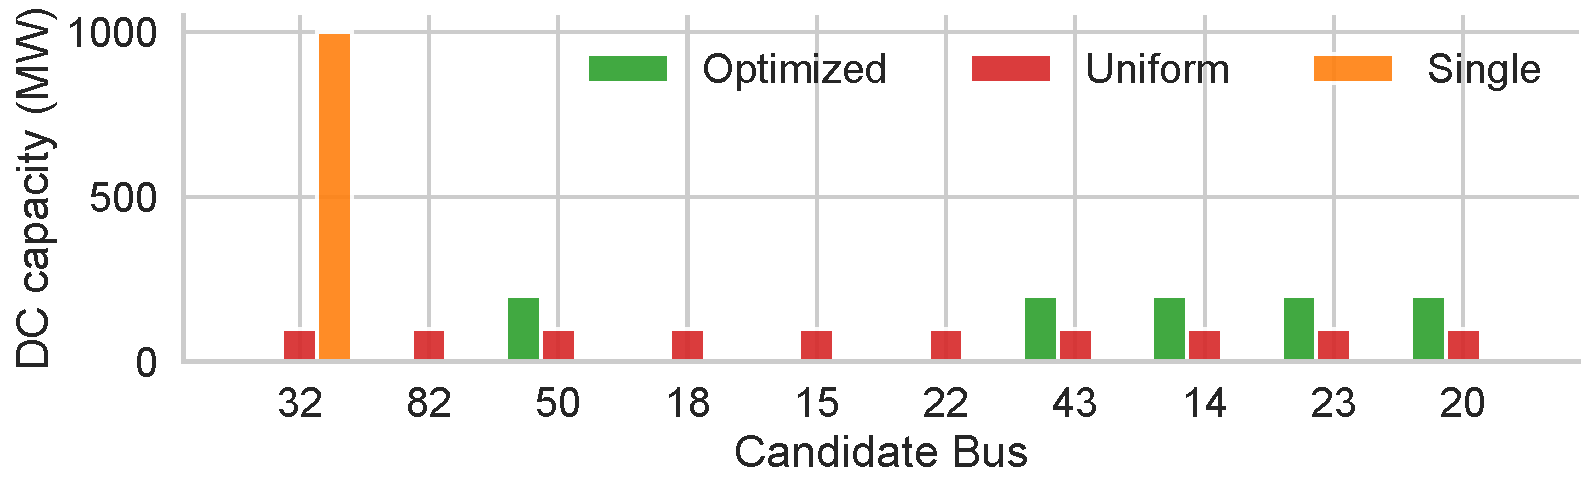
\includegraphics[width=\textwidth]{figures/dc_allocation_bar_plot-1.pdf}
    \caption{Planned data center capacity across candidate buses under different allocation policies.}
    \label{fig:dc_allocation_bar_plot}
  \end{subfigure}

  \begin{subfigure}[t]{\columnwidth}
    \centering
    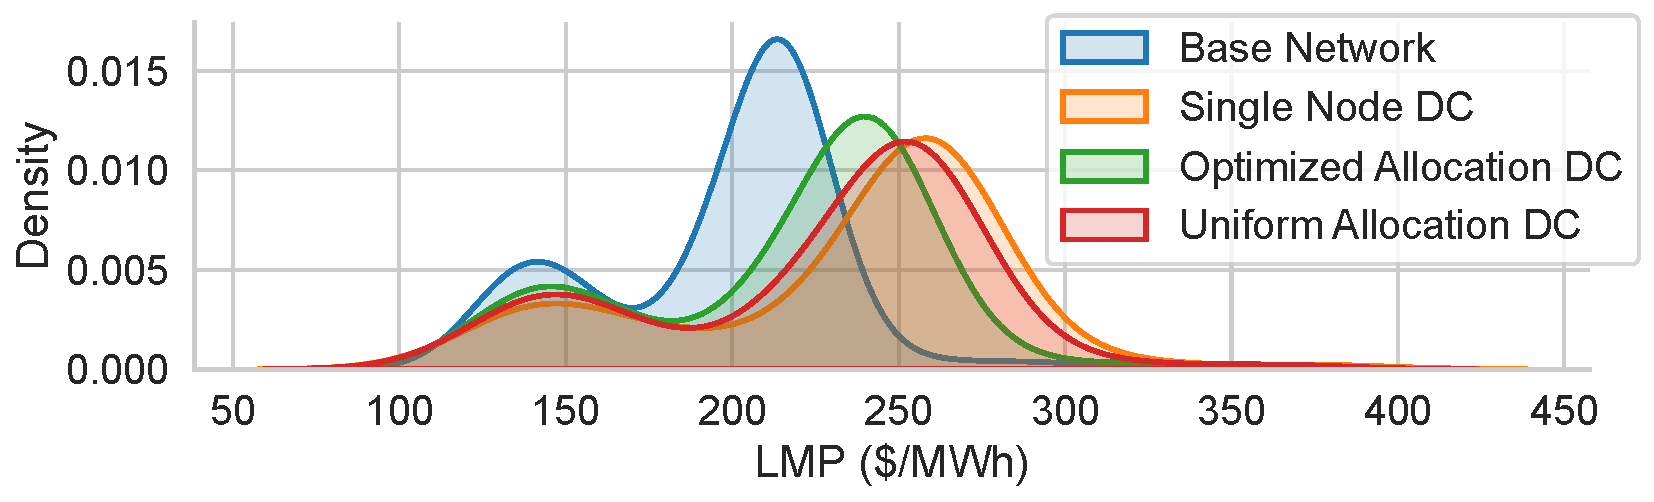
\includegraphics[width=\columnwidth]{figures/kde_p95_lmp-1.pdf}
    \caption{P95 of LMP across buses.}
    \label{fig:kde_p95_lmp}
  \end{subfigure}
  
  \vspace{0.6em}

  \caption{System LMP shifts risk and data center capacity allocation.}
  \label{fig:lmp_and_allocation}
\end{figure}

We first examine the impacts of distributing datacenter capacity as a load-side lever to manage grid impacts. To understand the base dispatch, we solve Problem (\ref{eq:dc-opf-full}) with no datacenter load added to the system. For the single node injection case, we build a single 1GW datacenter at the cheapest land cost node from the set of candidate buses selected according to the methodology in Section \ref{sec:candidate_selection}. To determine the optimized distributed allocation, we first fix $K=10$ buses from the candidate set. The minimum and maximum allowable datacenter capacities at each location are set to $\underline{\eta}=50$MW and $\overline{\eta}=250$MW respectively.  All candidate nodes utilize the inference workload profile. We then solve Problem (\ref{eq:dc_plan}) with 10 steps of projected gradient descent with $\alpha=20$, $\beta=1000$, and step size $s=0.01$. To determine the uniform allocation, we assign 100MW of capacity to each of the 10 nodes. In all cases where we provision datacenter capacity, we solve Problem (\ref{eq:dc-opf-full}) with the determined capacities at each of the specified buses to examine the LMPs and flows in the system. 

Figure \ref{fig:dc_allocation_bar_plot} shows the single node, uniform, and optimized allocations. The optimized allocation selects only a subset of the candidate nodes at which to allocate 200MW each. For each scenario, we compute the $95\textsuperscript{th}$ percentile LMP at each node over the 24 hour simulation window. Figure \ref{fig:kde_p95_lmp} shows the kernel density estimates for the spatial distribution of P95 LMPs at each bus. We observe that the optimized allocation pushes the P95 prices lower towards the base dispatch prices. Naive distribution as is done in the uniform case does not show substantial improvement over the single node injection. While not shown, we note that the distributions look similar when the temporal aggregation metric at each node is max or mean instead of the $95\textsuperscript{th}$ percentile. 

\subsection{Comparative Analysis of Levers}

We compare several expansion scenarios to assess how distributed datacenter placement performs relative to conventional grid-side levers. The single node and optimized distributed datacenter allocations are determined according to the methods in Section~\ref{sec:load_side_lever}. We then consider the same single node injection of 1~GW, but allow for either transmission or generation expansion. Finally, we consider the optimized distributed allocation with either transmission or generation expansion to demonstrate the combined effects of multiple levers.

For transmission expansion, we solve Problem~\eqref{eq:trans_plan} with $\mathcal{E} = \mathcal{E}_{\text{trans}}$ using 10 steps of projected gradient descent with step size $s = 0.01$, allowing up to a 5\% increase in transmission capacity per line. For generation expansion, we solve the analogous problem with $\mathcal{E} = \mathcal{E}_{\text{gen}}$, allowing up to a 2.5\% increase in capacity per generator. In both cases, the planning objective is $\gamma^\top \eta + h_{\text{dispatch}}$, reflecting that these are system upgrades where the grid operator seeks to minimize investment while reducing operational cost.

For combined scenarios, we first solve Problem~\eqref{eq:dc_plan} to determine the distributed datacenter allocation, then subsequently solve the transmission or generation expansion problem with the distributed capacity injected into the network. We optimize these sequentially rather than jointly due to the discrepancy in planning objectives. Transmission and generation are system upgrades planned to minimize investment and dispatch cost, whereas datacenter placement is not a system upgrade and may prioritize factors like LMPs that fall outside standard grid operator objectives. This separation also reflects realistic institutional constraints, where datacenter operators select sites based on their own objectives before grid operators plan responsive upgrades.

\paragraph{Metrics.}
For each scenario, we report annualized investment cost (M\$/yr) over a 20-year horizon with a 7\% discount rate, and dispatch cost (M\$/day) for the simulated day of operation. Given the matrix of nodal LMPs $\Lambda \in \mathbb{R}^{N \times T}$, we compute the following LMP metric: 
% {\setlength{\abovedisplayskip}{3pt}
%  \setlength{\belowdisplayskip}{3pt}
\begin{equation}
\mathrm{LMP} = \frac{1}{N}\sum_{n=1}^{N}\max_{t\in\{1,\dots,T\}} \Lambda_{n,t}.
\end{equation}
% }\noindent
which denotes the mean across nodes of the max LMP at each node over time. This serves as an interpretable proxy for the smooth-max objective used in optimization. To quantify congestion, we consider the shadow prices $\mu_\ell^+, \mu_\ell^-$ associated with the upper and lower transmission line flow constraints for each line $\ell$. At any timestep, at most one of these can be nonzero, so their sum captures the binding shadow price. We aggregate this as
\begin{equation}
    C = \frac{1}{L} \sum_{\ell=1}^{L} \max_{t \in \{1,\ldots,T\}} \left( \mu_\ell^+(t) + \mu_\ell^-(t) \right),
\end{equation}
which represents the average across lines of the peak shadow price over time. Table~\ref{tab:synopsis_tradeoffs_singlecol_ops} reports percentage change in this metric relative to the base scenario (no datacenter load).

\paragraph{Results.}
The results are summarized in Table~\ref{tab:synopsis_tradeoffs_singlecol_ops}. Distributing datacenter capacity across multiple sites reduces the LMP metric from 378.4~\$/MWh (single node) to 217.2~\$/MWh, yielding a 42.6\% reduction at nearly identical datacenter investment cost (1.21 vs.\ 1.19~M\$/yr). This LMP reduction is comparable to what is achieved by single-node injection paired with transmission expansion (216.6~\$/MWh), which requires 8$\times$ higher total investment (9.64~M\$/yr). Distribution also improves the congestion metric, reducing it from 24.66\% above base to 19.18\% above base.

Conventional grid-side levers, such as transmission and generation expansion, achieve similar LMP improvements but at substantially higher cost. Adding transmission capacity under single-node injection reduces congestion below the base scenario ($-4.11$\%), indicating that targeted upgrades can relieve pre-existing bottlenecks beyond offsetting the new load. Generation expansion reduces LMPs but is less effective at relieving congestion (14.38\% above base), consistent with the fact that added generation capacity does not directly alleviate transmission constraints.

The combined scenarios demonstrate that distribution and grid-side levers are complementary. Distributed placement paired with transmission expansion achieves the lowest LMP (202.4~\$/MWh) and congestion ($-7.08$\%) outcomes at similar cost to the single-node-plus-transmission case. This suggests that distributed siting improves the price response of the grid, allowing the same grid investment to go further. Notably, the transmission and generation expansions are modest relative to the datacenter load, adding 466--469~MW and 342--343~MW respectively against a 1~GW interconnection, yet yield meaningful improvements when combined with optimized placement.

Dispatch cost remains nearly constant across all scenarios (0.226--0.227~M\$/day). This is consistent with the observation that LMPs reflect local prices at constrained nodes, while dispatch cost captures total system operating cost. Congestion-induced redispatch affects prices at the margin, but if the volume of redispatched energy is small relative to total system load, aggregate dispatch cost may not shift substantially even as localized price spikes occur.

% To assess the efficacy of distributing provisioned datacenter capacity as a load-side lever relative to more conventional planning levers such as transmission and generation expansion, we run several expansion planning experiments and observe their impacts on various metrics. The single node and distributed datacenter allocation scenarios are determined according to the methods outlined in Section \ref{sec:load_side_lever}. We then consider the same single node injection of 1GW at a single site, but allow for either transmission or generation expansion as well. Finally, we consider the optimized distributed allocation of datacenter capacity and allow for either transmission or generation expansion to demonstrate the combined effects of using multiple levers in conjunction with each other. 

% In the single node datacenter case mitigated with transmission expansion, we solve Problem (\ref{eq:trans_exp}) using 10 steps of projected gradient descent with a step size of $s=0.01$. We allow for up to a $5\%$ increase in the transmission capacity of each line in the system. Similarly, for the single node case with generation expansion, we solve Problem (\ref{eq:gen_exp}) with the exact same algorithm parameters but allowing for up to $2.5\%$ increase in the capacity of each generator. 

% For the combined cases of distributed allocation in addition to transmission or generation expansion, we independently solve Problem (\ref{eq:dc_plan}) (as outlined in Section \ref{sec:load_side_lever}), and then subsequently solve either Problem (\ref{eq:trans_exp}) or (\ref{eq:gen_exp}) as specified above with the distributed capacity injected into the network. We choose \emph{not} to optimize datacenter capacity jointly with transmission or generation due to the discrepancy in planning objectives. The planning objective for transmission and generation expansion is $\gamma^{\top}\eta + h_{\text{dispatch}}$, while the datacenter expansion objective is only $h_{\text{LMP}}$. The transmission and generation expansion planning objectives reflect that these are \emph{system} upgrades in response to a large-load interconnection. While these upgrades may have been triggered by the load, the objective for the grid operator is to simultaneously minimize investment while reducing operational (dispatch) cost of the system. On the other hand, planning for datacenter capacity expansion is not a system upgrade, and thus there are various operational factors that may be important (like LMPs) that are outside the purview of standard grid operator objectives. 

% The results are summarized in Table \ref{tab:synopsis_tradeoffs_singlecol_ops}. For each scenario, we report the total investment cost (i.e. the sum of generation, transmission, and datacenter costs) as an annualized cost in M\$\slash yr. The dispatch cost for the 24 hour simulation window is also reported in M\$ \slash yr. Given the matrix of nodal LMPs $\Lambda \in \mathbb{R}^{N \times T}$, we compute the Table \ref{tab:synopsis_tradeoffs_singlecol_ops} metric ``LMP'' as 
% {\setlength{\abovedisplayskip}{3pt}
%  \setlength{\belowdisplayskip}{3pt}
% \begin{equation}
% \mathrm{LMP} = \frac{1}{N}\sum_{n=1}^{N}\max_{t\in\{1,\dots,T\}} \Lambda_{n,t}.
% \end{equation}}\noindent
% which denotes the mean across nodes of the max LMP at each node over time. 

% - explain the LMP metric
% - LMP result (distribution helps)
% - other levers help a similar amount but are way more expensive
% - in the combined case, distribution helps to push the LMPs down much more for a similar cost as to just transmission or generation. 

% - write down transmission line flow constraints
% - define the duals of mu+ and mu- of the transmission line flow constraints
% - define how we use those to form the congestion metric 
% - given an interpretation of the metric
% - explain that all results are reported relative to base (which is 0)
% - congestion result (distribution helps)
% - other levers help as well, and actually more. 
% - explain why this makes sense in the case of transmission expansion
% - explain how the combined case seems to help even more than just individual


% - note that dispatch cost doesn't seem to be changing much
% - explain why dispatch cost is not changing much 


\begin{table}[t]
\centering
\renewcommand{\arraystretch}{1.15}
\caption{Synopsis of planning tradeoffs across siting scenarios. Total investment cost (M\$/yr) are annualized over a 20yr period with a 7\% discount rate and dispatch costs (M\$/day) are calculated for the day of operation. LMPs are in \$\slash MWh. Congestion is \% change from the base scenario. }
\label{tab:synopsis_tradeoffs_singlecol_ops}
\resizebox{\columnwidth}{!}{
\begin{threeparttable}

\begin{tabular}{lccccccc}
\toprule
\textbf{Scenario} &
\textbf{Gen.} &
\textbf{Tx.} &
\textbf{DC} &
\textbf{Total} &
\textbf{LMP} &
\textbf{Dispatch} &
\textbf{Rel. Congestion} \\
\midrule
Base Case        & ---   & ---   & ---  & ---  & 196.78 & 0.225 & 0 \\
Single node (SN)        & ---   & ---   & 1.19 & 1.19 & 378.4 & 0.227 & 24.66 \\
Distributed (Dist)      & ---   & ---   & 1.21 & 1.21 & 217.2 & 0.227 & 19.18 \\
SN + transmission       & ---   & 8.45  & 1.19 & 9.64 & 216.6 & 0.227 & -4.11 \\
SN + generation         & 18.98 & ---   & 1.19 & 20.17 & 215.7 & 0.226 & 14.38 \\
Dist + transmission     & ---   & 8.48  & 1.21 & 9.69 & 202.4 & 0.226 & -7.08 \\
Dist + generation       & 19.18 & ---   & 1.21 & 20.38 & 205.0 & 0.226 & 8.22 \\
\bottomrule
\end{tabular}

\begin{tablenotes}[flushleft]\footnotesize
\item \textit{Notes:} ``+ transmission'' allows transmission expansion up to 5\% (added 466--469\,MW). ``+ generation'' allows generation expansion up to 2.5\% (added 342--343\,MW).
\end{tablenotes}
\end{threeparttable}
}
\end{table}


\section{Budget and Site Count Constraints}


\section{Workload Impacts on Placement}








% \section{Planning for Diverse Workloads}

\section{Related Works}

\noindent\textbf{Geographic load balancing.}
Since the onset of cloud-based computing, geographic load balancing has been proposed as a way to balance compute across multiple regions towards lowering electricity prices and carbon intensity~\cite{qureshi2009cutting,liu2015greening}.
Within this GLB framing, work incorporates intermittency by coupling load shifting with renewable generation, storage, and backup-grid usage~\cite{liu2011geoloadbalance,goiri2011greenslot,berral2014buildinggreencloud}.
More broadly, “green cloud” control planes combine request routing, VM migration, admission control, and storage-aware scheduling to improve renewable utilization or reduce cost/carbon emissions~\cite{zhang2011greenware,radovanovic2023carbonaware, johnson2025signalawareworkloadshiftingalgorithms}.

\noindent\textbf{Grid-aware datacenter siting and placement.}
A smaller set of work directly couples datacenter siting decisions to power-system feasibility, moving beyond site-local signals to include transmission-network effects.
These models capture how placement choices interact with congestion, losses, and operational constraints (e.g., line overload and voltage violations)~\cite{goiri2011intelligentplacement,wang2015griddcwind}.
By embedding grid physics into the placement objective and constraints, this line motivates treating datacenters as grid-sited assets whose system-level impacts depend on \emph{where} capacity is added, not just on total demand.

\noindent\textbf{Datacenters for demand response.}
Complementary work studies datacenters as controllable demand capable of providing flexibility through policy-driven load modulation, workload shifting, and local generation/storage~\cite{irwin2011continuousdr,liu2013coincidentpeak}.
This literature primarily targets \emph{operational} coupling (minutes to hours), characterizing which forms of datacenter flexibility are practical, what signals they can respond to, and how these choices interact with utility cost structures and grid stress.

\noindent\textbf{Capacity Expansion Modeling Tools}
Grid-aware planning relies on optimization frameworks to explore new situations under uncertainty.
PyPSA and PyPSA-USA enable network-constrained, multi-period studies with renewables and storage~\cite{PyPSA,tehranchi5029120pypsa}, while capacity-expansion platforms such as SWITCH, Calliope, and oemof support multi-decade planning with high renewable penetration~\cite{nelson2012switch,johnston2019switch2,pfenninger2018calliope,hilpert2018oemof}.
Bilevel and expansion-planning formulations are well established in power systems~\cite{baringo2011wind}. Gradient-based methods can maker multi-scenario expansion planning scalable to larger problem sizes~\cite{degleris2024gradient,degleris2024gpu}.

\input{conclusion}

% \section*{Acknowledgment}

\bibliographystyle{ACM-Reference-Format.bst}
\bibliography{sample-base}

\end{document}